% This template has been tested with LLNCS DOCUMENT CLASS -- version 2.20 (24-JUN-2015)

%"runningheads" enables:
%  - page number on page 2 onwards
%  - title/authors on even/odd pages
%This is good for other readers to enable proper archiving among other papers and pointing to
%content. Even if the title page states the title, when printed and stored in a folder, when
%blindly opening the folder, one could hit not the title page, but an arbitrary page. Therefore,
%it is good to have title printed on the pages, too.
\documentclass[runningheads,a4paper]{llncs}[2015/06/24]

%cmap has to be loaded before any font package (such as cfr-lm)
\usepackage{cmap}
\usepackage[T1]{fontenc}

\usepackage{graphicx}

% für neue deutsche Rechtschreibung
%\usepackage[english,ngerman]{babel}

% für englische Rechtschreibung
%Even though `american`, `english` and `USenglish` are synonyms for babel package (according to https://tex.stackexchange.com/questions/12775/babel-english-american-usenglish), the llncs document class is prepared to avoid the overriding of certain names (such as "Abstract." -> "Abstract" or "Fig." -> "Figure") when using `english`, but not when using the other 2.
%english has to go last to set it as default language
\usepackage[ngerman,english]{babel}

%Eingabeformat UTF-8
\usepackage[utf8]{inputenc}

%Hint by http://tex.stackexchange.com/a/321066/9075 -> enable "= as dashes
\addto\extrasenglish{\languageshorthands{ngerman}\useshorthands{"}}

%cfr-lm is preferred over lmodern. Reasoning at http://tex.stackexchange.com/a/247543/9075
\usepackage[%
rm={oldstyle=false,proportional=true},%
sf={oldstyle=false,proportional=true},%
tt={oldstyle=false,proportional=true,variable=true},%
qt=false%
]{cfr-lm}
%
%if more space is needed, exchange cfr-lm by mathptmx

\graphicspath{{graphics/}}

%Tweaks by IPVS/AS
\usepackage{lncs_as}

%for demonstration purposes only
\usepackage[math]{blindtext}

%Sorts the citations in the brackets
%It also allows \cite{refa, refb}. Otherwise, the document does not compile.
%  Error message: "White space in argument"
\usepackage{cite}


%% If you need packages for other papers,
%% START COPYING HERE
%% COPY ALSO cmap and fontenc from lines 10 to 12

%extended enumerate, such as \begin{compactenum}
\usepackage{paralist}

%put figures inside a text
%\usepackage{picins}
%use
%\piccaptioninside
%\piccaption{...}
%\parpic[r]{\includegraphics ...}
%Text...

%for easy quotations: \enquote{text}
\usepackage{csquotes}

%enable margin kerning
\usepackage{microtype}

%tweak \url{...}
\usepackage{url}
%\urlstyle{same}
%improve wrapping of URLs - hint by http://tex.stackexchange.com/a/10419/9075
\makeatletter
\g@addto@macro{\UrlBreaks}{\UrlOrds}
\makeatother
%nicer // - solution by http://tex.stackexchange.com/a/98470/9075
%DO NOT ACTIVATE -> prevents line breaks
%\makeatletter
%\def\Url@twoslashes{\mathchar`\/\@ifnextchar/{\kern-.2em}{}}
%\g@addto@macro\UrlSpecials{\do\/{\Url@twoslashes}}
%\makeatother

%diagonal lines in a table - http://tex.stackexchange.com/questions/17745/diagonal-lines-in-table-cell
%slashbox is not available in texlive (due to licensing) and also gives bad results. This, we use diagbox
%\usepackage{diagbox}

%required for pdfcomment later
\usepackage[hyperref,svgnames]{xcolor}

\usepackage{listings}
\lstloadlanguages{java}
\lstset{language=java,numbers=left,captionpos=b}


%enable nice comments
%this also loads hyperref
\usepackage{pdfcomment}
%enable hyperref without colors and without bookmarks
\hypersetup{hidelinks,
   colorlinks=true,
   allcolors=black,
   pdfstartview=Fit,
   breaklinks=true}
%enables correct jumping to figures when referencing
\usepackage[all]{hypcap}

\newcommand{\commentontext}[2]{\colorbox{yellow!60}{#1}\pdfcomment[color={0.234 0.867 0.211},hoffset=-6pt,voffset=10pt,opacity=0.5]{#2}}
\newcommand{\commentatside}[1]{\pdfcomment[color={0.045 0.278 0.643},icon=Note]{#1}}

%compatibality with packages todo, easy-todo, todonotes
\newcommand{\todo}[1]{\commentatside{#1}}
%compatiblity with package fixmetodonotes
\newcommand{\TODO}[1]{\commentatside{#1}}

%enable \cref{...} and \Cref{...} instead of \ref: Type of reference included in the link

%\usepackage[capitalise,nameinlink,ngerman]{cleveref}
\usepackage[capitalise,nameinlink,english]{cleveref}
%Nice formats for \cref - only for English texts
%\crefname{section}{Sect.}{Sect.}
%\Crefname{section}{Section}{Sections}

\usepackage{xspace}
%\newcommand{\eg}{e.\,g.\xspace}
%\newcommand{\ie}{i.\,e.\xspace}
\newcommand{\eg}{e.\,g.,\ }
\newcommand{\ie}{i.\,e.,\ }

%introduce \powerset - hint by http://matheplanet.com/matheplanet/nuke/html/viewtopic.php?topic=136492&post_id=997377
\DeclareFontFamily{U}{MnSymbolC}{}
\DeclareSymbolFont{MnSyC}{U}{MnSymbolC}{m}{n}
\DeclareFontShape{U}{MnSymbolC}{m}{n}{
    <-6>  MnSymbolC5
   <6-7>  MnSymbolC6
   <7-8>  MnSymbolC7
   <8-9>  MnSymbolC8
   <9-10> MnSymbolC9
  <10-12> MnSymbolC10
  <12->   MnSymbolC12%
}{}
\DeclareMathSymbol{\powerset}{\mathord}{MnSyC}{180}

% correct bad hyphenation here
\hyphenation{op-tical net-works semi-conduc-tor}

%% END COPYING HERE


\begin{document}

\title{Apache Storm}
%If Title is too long, use \titlerunning
%\titlerunning{Short Title}

\author{Aanal Raj Basaula}

\supervisor{Matthias Wieland}

\seminar{Advanced Topics in Data Management}

\semester{WS 2017/2018}

\abgabedatum{Stuttgart, 11.12.2017}

\institute{\email{aanal.basaula@gmail.com}}

%\frontpagede % creates the frontpage (in German)
\frontpageen % creates the frontpage (in English)

\thispagestyle{empty}
\cleardoublepage

\maketitle

\begin{abstract}
Apache Storm is one of the available open source tools for Stream Data Processing. This document provides a brief overview of the intricacies of the Architecture of Storm and tends to proceed further on the details of considerations required to design a Solution based on Storm. The design considerations relating to deployment of Storm System as a Lambda or a Lambda-less Architecture and the sketch of the various internal components of Storm i.e. Bolts, Spouts. We consider a practical implementation of Storm to try and express the theoretical design considerations in practice. Finally we list out the other available tools and compare them to Storm with regard to Performance, Resilience and various other parameters.
\end{abstract}

\begin{keywords}
Apache Storm, Stream Processing, Real Time Processing, Big Data
\end{keywords}

\section{Introduction}

\textbf{Data} today is generated by a lot of devices that are connected to the internet and the amount of data being generated at any instance is increasing rapidly. These devices could include a personal computer, a smart phone, or even an embedded device. Due to the rapid adoption of Internet of Things, data is being generated at an unprecedented rate. The sheer volume of data generated and the rate at which it is being generated can be termed as Big Data. \textbf{Big Data} made it's appearance in 1998 SGI slide by John Mashey and now is of interest to a lot of financial as well as research institutions.\cite{miningstatus}

Data can be considered the oil of this present age, because with huge amounts of data one can determine hidden patterns. A lot of companies utilize pattern recognition on big data to open opportunities for revenue generation whereas research institutions use it to discover patterns simply not observable by the human mind(simply due to the volume of data). The question on how to classify any data as big data can be answered by using the 3Vs: Volume, Variety and Velocity \cite{usingapachestorm}. Any data with big volume or variety (such as text, video, images, etc) or that gets generated rapidly can be considered as big data. In this paper regarding \textbf{Apache Storm} we consider the third V of big data to be the influencing factor.

\textbf{Data Stream} is a sequence of data flowing from a source to a destination, for example a sensor reporting the temperature to a server. The sensor measures the temperature periodically and updates it to the server. Another example could also be the purchase requests of products in a shopping site. In all of these scenarios, the data is continuously being generated. Traditionally analyzing of these types of data requires storage of these data onto persistence and later batch processing it to discern patterns as well as other useful information. But, with the help of \textbf{Apache Storm} we are able to process these data as they are generated with minimum amount of latency.

This benefit could be a major game changer for many companies as Stream processing of data allows Real Time Analysis. As an example, an online store could monitor its purchase requests for best performing and least performing articles and could offer discounts on the articles not performing good to increase their sales volume. This small change could increase the gross income of a company and will surely be advantageous.

\section{Apache Storm: Concepts}
\label{sec:concepts}

Apache storm is one of the available open source tools for stream data processing, which is considered to be one of the most easy to use, fast and fault tolerant systems available \cite{stormperspective}. These three factors have been the major points for the general public to choose \textbf{Apache Storm} above other available tools. It was originally created by Nathan Marz at BackType and till now, at present more than 60 companies use or experiment with this tool.

\subsection{Architecture Overview}
The basic Storm data processing architecture consists of stream of tuples flowing through a defined topology to yield the required analytic result. Processing of this stream data is performed in Nodes called the worker nodes, which are responsible for performing the required calculations. There is also another node named the Master Node, which is responsible for the complete Storm infrastructure,  by keeping track of all the worker nodes and the total topology itself.

\begin{figure}
  \begin{center}
    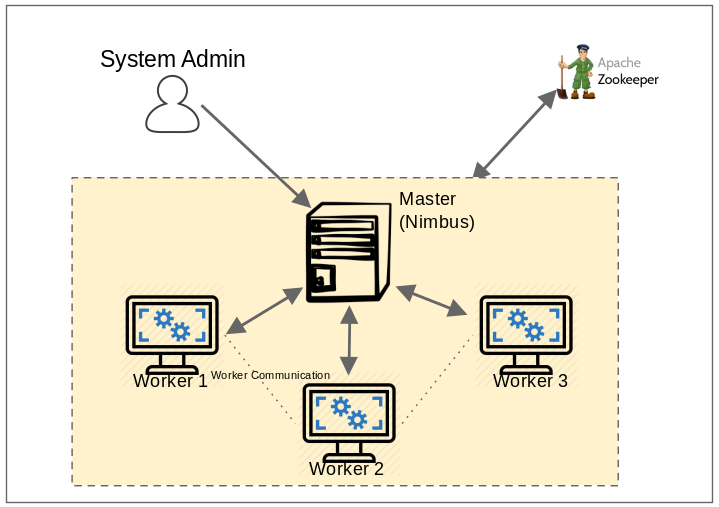
\includegraphics[width=.7\textwidth]{arch.png}
    \caption{High Level Storm Architecture}
    \label{fig:arch}
   \end{center}
\end{figure}

\subsubsection{Nimbus}

\paragraph{The Master node} also called the \textbf{Nimbus} is also responsible for distribution and coordination of the execution of topologies. The Nimbus is the first point where the user submits the defined topology, which is then distributed among the worker nodes.  Figure \ref{fig:arch} illustrates the high level architecture where, Nimbus monitors all the available worker nodes and both the nimbus as well as the worker nodes use \textbf{Apache Zookeeper} to store their states. The actual processing is done by the \textbf{worker nodes}, and each worker node runs multiple Worker Processes each of them mapped to their own topology \cite{stormtwitter}. It is also worth while noting that multiple worker processes in a worker node could be executing different parts of the topology.

\subsubsection{Worker Node}
\paragraph{Worker Node} is responsible for all the heavy lifting required for processing of the topology. One worker node may run a multiple number of worker processes. Each of these worker processes may belong to the same topology or different topologies. A worker node maintains a \textbf{Supervisor} and a multiple number of Worker Processes which in turn maintains a multiple number of executors. Thus, Executors enable intra-topology parallelism whereas Tasks provide intra-spout or intra-bolt parallelism. Figure \ref{fig:workerarch} depicts the design of a Worker node.\cite{stormtwitter}

\begin{figure}
  \begin{center}
    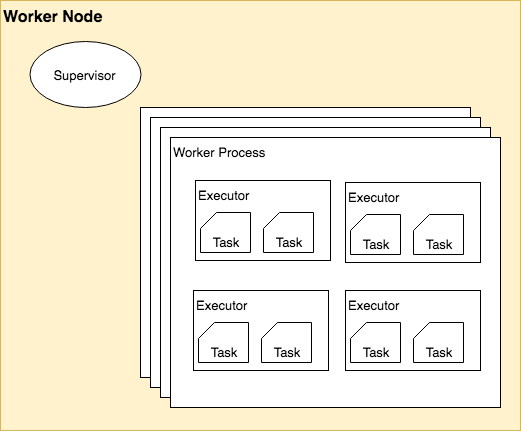
\includegraphics[width=.7\textwidth]{worker.png}
    \caption{Worker Node Architecture}
    \label{fig:workerarch}
   \end{center}
\end{figure}

\paragraph{Supervisor} is running in every Worker Node and communicates with the Nimbus to receive assignments from it. Apart from taking assignments from the Nimbus it is also responsible for monitoring the health of the of the worker processes and respawns the worker processes in case it dies.

\paragraph{Worker Process} is the Entity that does the processing and is mapped to a certain topology. Each worker node spawns a JVM and runs one or multiple executors. These executors may be running any of the bolt or spout within the topology, thus providing an added level of parallelism.

\paragraph{Executors} are made up of one or multiple Tasks. Unless specified explicitly, storm assigns single task to a single executor. Executors takes tuples from the in queue, examines the task this tuple is destined to, performs the task and then places the result in the out queue \cite{stormtwitter}.

\subsection{Topology}
\paragraph{Topology} is a directed graph where the vertices represent computation and the edges represents the data flow. Another important thing about topologies in Storm is that they are allowed to have cycles. Figure \ref{fig:topo} shows a basic Storm Topology, which consists of Spouts and Bolts. Spouts are the Sources of tuples in a Topology whereas Bolts are the units which process these generated tuples. The user first submits the topology to the Apache Storm Nimbus, which consults with each of the available Supervisors in the worker nodes and assigns each of them with tasks related to the topology.

\subsubsection{Spout} 
\paragraph{Spouts} are the entry point for any data in the Storm Topology. As shown in the figure \ref{fig:topo} spouts take data from external source and emits them into the topology as tuples. The input source could be a Heterogenous data source.

\subsubsection{Bolt} 
\paragraph{Bolts} are the processing entities of a Topology. It receives raw tuples emitted by spouts or processed tuples sent by another bolt and sends it down the pipe after it has completed its processing.

\begin{figure}
  \begin{center}
    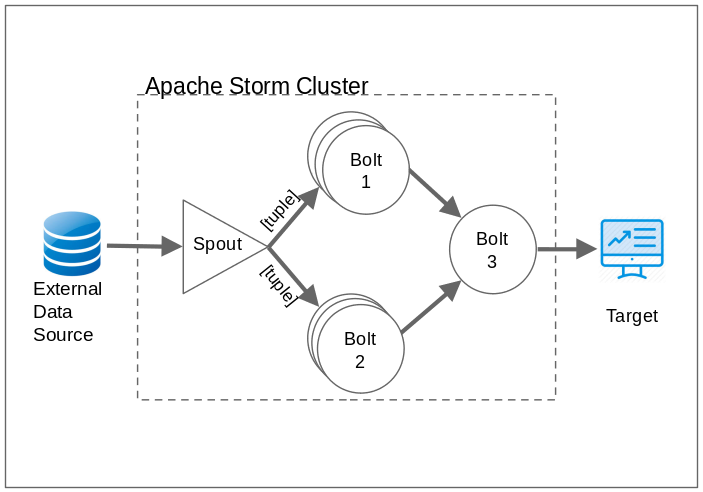
\includegraphics[width=0.85\textwidth, height= 0.23\textheight]{topo.png}
    \caption{Generic Storm Topology}
    \label{fig:topo}
   \end{center}
\end{figure}

\subsection{Fault Tolerance and Resilience}
\label{sec:resilience}
Apache storm offers fault tolerance and resilience mechanisms with out of the box support and is tolerant against different types of failures. Nimbus, being the main master node, is in-charge of all the other worker nodes. Under the circumstance that a worker node fails, Nimbus re-spawns a worker node and assigns the tasks to this node. If the nimbus itself fails, the nimbus is not re-started automatically, but the worker nodes do not stop processing the stream. The nimbus can be later on restarted manually. During this phase, if a worker fails, it will not be restarted. The supervisor is also an active element within the Storm Architecture and keeps the Nimbus posted about it's current status. The \textbf{heartbeat} event is scheduled to run every 15 seconds and it reports to the Nimbus that the worker node is alive. \cite{stormtwitter}

\begin{figure}
  \begin{center}
    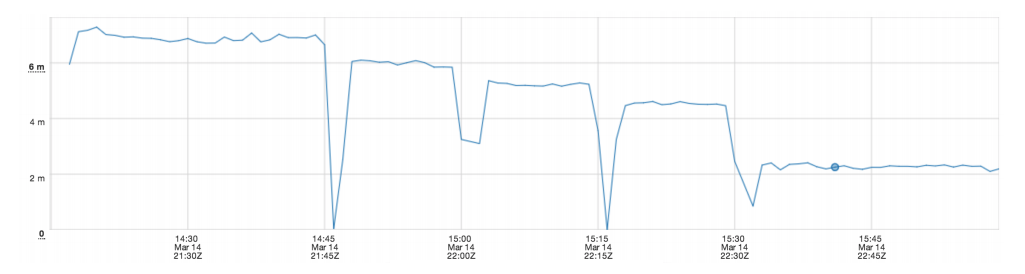
\includegraphics[width=\textwidth, height=0.25\textheight]{throughput.png}
    \caption{Throughput in time with respect to changing worker node availability \cite{stormtwitter}}
    \label{fig:throughput}
   \end{center}
\end{figure}

As we can see in figure \ref{fig:throughput}, an experiment conducted in \cite{stormtwitter} to check the resilience and performance of storm under loss of worker nodes. The worker nodes were turned off one by one in fixed durations, and the throughput of the system was measured at every instance. The durations and number of machines are shown below in table \ref{tab:experiment}. As seen, 3 machines were killed every 3 minutes, but the number of workers were limited to 50 at every instance, thus increasing the number of workers per machine. The graph \ref{fig:throughput} suggests that every 15 minutes, when the worker nodes were killed, the throughput was reduced significantly while storm tries to balance the topology again. The balancing does not require extensible amount of time and results into a new maximum throughput. As we can observe in the graph, the throughput decreses every time a node is removed, which is an expected phenomenon, due to the decrease in the computational capacity.

\begin{table}
\caption{Experimental setup during different time frames}
\label{tab:experiment}
\begin{center}
\begin{tabular}{r@{\quad}cl}
\hline
\multicolumn{1}{l}{\rule{0pt}{12pt} 
	Time}&\multicolumn{1}{l}{no of machines}\\[2pt]
\hline\rule{0pt}{12pt}
0 minutes  & 16  \\
+15 minutes & 13 \\
+30 minutes & 10 \\
+45 minutes & 7 \\
+60 mintues & 4 \\[2pt]
\hline
\end{tabular}
\end{center}
\end{table}

Apache Storm supports two types of processing schemes, \textbf{at least once} where each tuple is processed as the name suggests, at least once, and the other \textbf{at most once}, where the tuples are either processed once or dropped in cases of failure. To provide \textbf{at least once} semantics, Storm maintains an acker bolt, which keeps track of the tuple flow in the directed acyclic graph.

\begin{figure}
  \begin{center}
    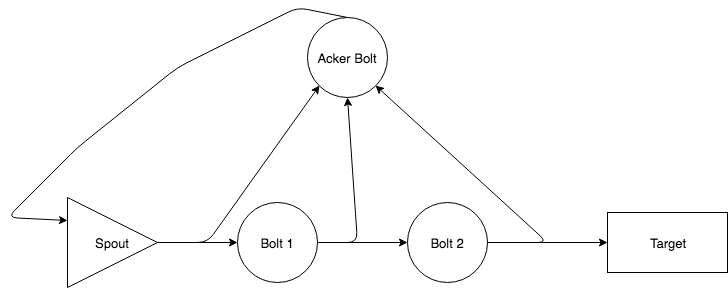
\includegraphics[width=.7\textwidth]{acker.png}
    \caption{Storm Acker Bolt \cite{stormtwitter}}
    \label{fig:acker}
   \end{center}
\end{figure}

\paragraph{Figure} \ref{fig:acker} shows the Acker bolt integration with the storm topology. It keeps track of the tuple flow starting from the point where it has been injected into the topology till it leaves the topology. After the tuple has left the topology, an \textbf{ack} is sent to the Spout, at this point, it can decide to remove the Tuple from memory.

	\section{Stream Processing: Design Considerations}
A stream is a continuous flow of data from one point to the another. A Stream Processing system works on these data streams, the work may just be simple transformations, but also could be as complex as predictive analysis. A stream processing system depending on the nature of application has different requirements.

Let us consider the news feed service provided by any social networking site, we know that in any of these websites we can read posts created by our friends or family and it does not matter if we see them at the very instance they post. But, there are cases such as a stream of purchases, where we want the data to be visible as soon as available separate design considerations should be made. This section focuses on the various considerations that are to be made while designing a stream processing system, specifically using Apache Storm.

\subsection{System Architecture}
As discussed above, a data processing stream has different requirements and according to these various requirements, the System can be modified to suit the needs. The major two System architectures currently available are the Lambda Architecture and the Lambda-less (or Kappa) Architecture.

\subsubsection{Lambda-less Architecture}
\paragraph{Kappa Architecture} or the lambda-less Architecture is a System Architecture concept where there are only two layers, namely Speed Layer and Serving Layer.The data input to the system is processed at real time to retrieve the results at real time. The major advantage of this type of system is that there is minimum latency. This type of architecture is more suitable in cases where an accurate view of the data is preferable without a lot of delay. Cash transactions might be one of these cases where a minimum delay for transaction visualization is suitable added the calculations done on these data sets are properly formulated as well.

This architecture can be considered has an advantage over the lambda architecture (described later) , that a single code base is to be maintained throughout the life of the software. But, any apparent change to the code base results in a need for a duplicate cluster to analyze the data again and update the view. A working example of this architecture is presented in the section \ref{sec:usecase}. One may use this architecture over the lambda architecture when both the algorithms for the batch processing and stream processing are the same and the requirements mentioned above are the major focus.

\subsubsection{Lambda Architecture}
\paragraph{Lambda Architecture} is a data processing Architecture designed to handle high volume data utilizing the best of both batch and stream processing. Figure \ref{fig:lambda} shows a generic architecture principle for Lambda Architecture. The three composed layers are: Speed Layer, Batch Layer and Serving Layer. The batch processing layer provides an accurate view of the data but provides results in batches, whereas the speed layer provides current data visualizations which may or may not be accurate depending upon the algorithm. The serving layer utilizes both the speed layer as well as the batch layer to fulfill the request to a query.

Lambda architecture requires maintanence of two separate systems as well as code bases, and thus may result in higher cost. But, the added advantage is that the batch processing layer code can be optmized for the given data set to obtain better results. An example scenario could be a specialized news feed which requires machine learning algorithms to customize the user experience. The Speed layer could be used to deliver recent news, but the batch layer could use machine learning to produce the customized feed. An added advantage is that Lambda architecture holds the input data unchanged.\cite{lambdastorm}

\begin{figure}
  \begin{center}
    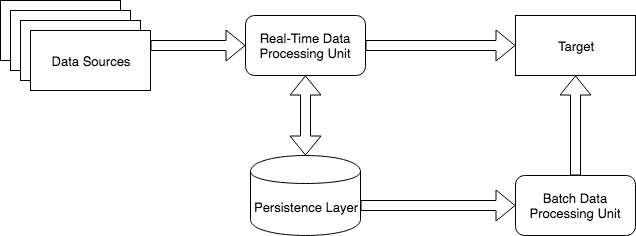
\includegraphics[width=.7\textwidth]{lambda.png}
    \caption{Lambda Architecture}
    \label{fig:lambda}
   \end{center}
\end{figure}

\subsection{Topology Design Considerations}
A storm topology design with the spouts and bolts and affects the overall system thus should be properly considered. A spout should inject data into the topology from external sources where as the bolt should be a smallest implementable task. A storm topology should also be considered with various considerations in mind:

\subsubsection{Scalability:} A designed topology should be considered with scalability in mind. The major question is what configuration of bolts enables us to process greater amount of data at real time. Let us consider a simple example of word count topology which counts the repetition of words and ranks the most used words. It can be performed by simply including a spout and two bolts, the first of which to count the number of words and the second to aggregate and rank it (see fig. \ref{fig:ranking} Topology Setup 1).
Since we should have only one instance of Aggregator, to be able to get the aggregated result, in cases of increased data load, the number of rolling count bolts can be increased, but the Aggregation Bolt cannot be increases thus adding increased load at this node. To relax the demand on this node, we can introduce another bolt, the Intermediate Ranking Bolt, which is responsible for ranking the words at a certain predefined intervals and passes the intermediate ranks to the aggregator. This reduces load on the Aggregator since we can increase the intermediate ranking bolts to cope with the increased load.

\begin{figure}
  \begin{center}
    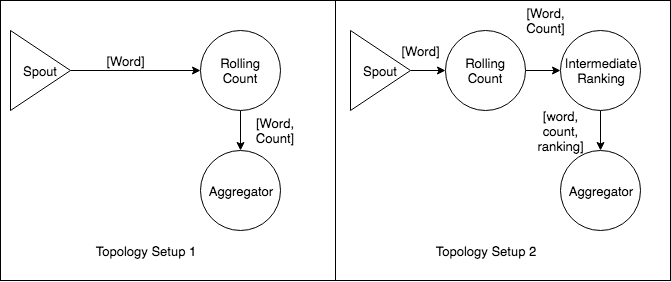
\includegraphics[width=\textwidth]{ranking.png}
    \caption{Possible Topologies for Word Count and Ranking}
    \label{fig:ranking}
   \end{center}
\end{figure}

\subsubsection{Resilience:} Apache storm includes APIs which allow users to develop solutions which are resilient in nature. Using the acker bolt as show in figure \ref{fig:acker}, users can track the progress of the tuple injected into the system. Thus, writing a spout which can replay the tuple in case of failures allows us to guarantee the processing of data. For additional details please follow Section \ref{sec:resilience}.

\subsubsection{Interoperability:} The designed topology should be interoperable with different sources of data, and by default should work out of the box by adding simply other Spouts in the topology. This also amounts to the maintainability of the code.

\section{Practical Use Case}
\label{sec:usecase}
Apache Storm is used for stream processing of data, in many sources [2,3] a word frequency count example has been shown which can be considered to be trivial, but in actual practice it can be used to execute complicated algorithms. For the purposes of this paper we consider a trivial but different example of \textbf{Sentiment Analysis}.

\subsection{Scenario}

\subsubsection{Description}
\paragraph{Let us consider} a company which produces a range of products, for example \textbf{Apple Inc.} produces IPhones, IPods, MacBooks, etc. For such a big company an understanding of the sentiment of the people is important to maintain a positive outlook. The company can also analyze the feedback people place on a specific product, to change and adjust the pricing schemes in real time to the demand.  At present there are many social media networks available and people tend to share their views on these networks,  \textbf{Twitter} is also one of these social networks where a number of posts are available publicly and can be analyzed to obtain a generalized view about a specific product or the company in general.

\subsubsection{Proposed Solution}

\paragraph{Solution} to the scenario can be implemented using \textbf{Apache Storm} to process the tweets in real time. Figure \ref{fig:solution} shows the simplified system overview, consisting of Twitter Streaming Servers as the source of information. This information is processed in the Storm Clusters from within the Company Infrastructure and the analyzed result is reported to the User Interface, which can be accessed by the appropriate user.

\begin{figure}
  \begin{center}
    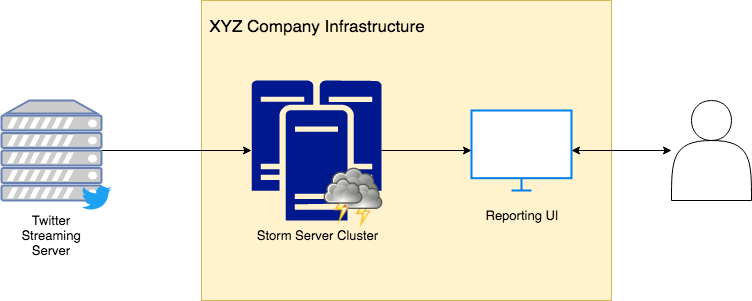
\includegraphics[width=.7\textwidth]{solution.png}
    \caption{Generic Streaming Solution implemented in this use case}
    \label{fig:solution}
   \end{center}
\end{figure}

\paragraph{This} is not the only possible solution, there are multiple other tools such as \textbf{Spark Streaming}, \textbf{Samza}, etc. but this paper considers Apache Storm as it is in the spotlight of this paper, for further details regarding other available tools and their comparisons with Apache Storm, please consider the section \ref{sec:othertools} for further details.

\subsection{Practical Implementation}
The implementation of this solution concluded in three sub phases, namely Design, Development and Deployment. In the design phase, the storm topology was thoroughly planned, specifically the spouts, bolts and how they are interconnected. In the development phase, these spouts, bolts and other required aspects of the software was programmed and lastly was deployed on a locally hosted storm server.

\subsubsection{Design}
\paragraph{Designing} a storm topology consists of determining the external sources of data (spouts), the processing that is required to this data imported from external sources (bolts) and the target system. Refer to figure \ref{fig:topoimpl} for the specific topology implementation for our use case. The sources of information for the scope of this paper is only Twitter Streaming API therefore a single Spout for integrating with the Twitter API is sufficient.

To Process the stream of tweets, we need to parse these tweets injected into the topology. The ParseTweetBolt processes these tweets and then emits whether the tweet was positive or negative under the simplified scenario. These separate positive or negative remark on a tweet does not provide useful information unless it is aggregated, thus a ResultAggregationBolt is responsible for aggregating all the results of the Parser bolt and providing the result to the target in real time.

\begin{figure}
  \begin{center}
    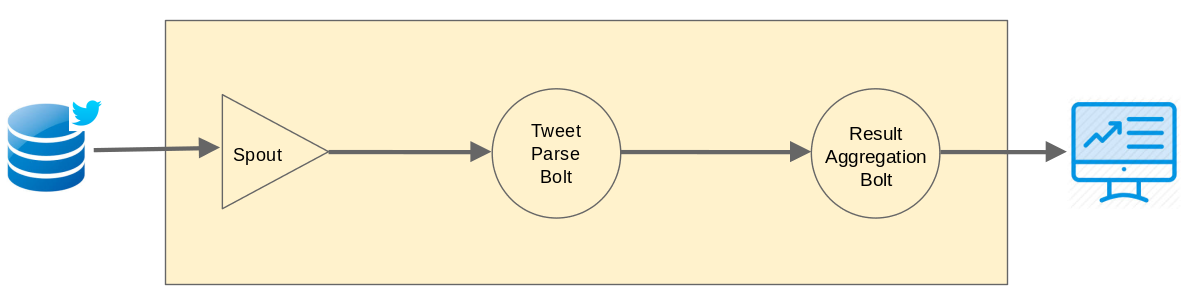
\includegraphics[width=.7\textwidth]{topoimpl.png}
    \caption{Topology Implementation for Sentiment Analysis}
    \label{fig:topoimpl}
   \end{center}
\end{figure}

The tweet spout contacts the twitter streaming server and fetches the available tweets in real time and relays it into the topology as a single tweet per tuple. The tuple is forwarded to the TweetParseBolt which will logically analyze the tweet as a positive or a negative tweet and with the percentage probability and emits this result to the ResultAggregationBolt. The ResultAggregationBolt calculates simply the weighted mean of the positive feedback and the negative feedbacks and outputs it into a local file, which can be later observed.

\subsubsection{Development}
\paragraph{Writing} code for storm can be achieved by using different programming languages depending upon the user. Apache Storm was designed to be usable with any programming languages\footnote{\url{http://storm.apache.org/about/multi-language.html}} and currently has Adapters available for Ruby, Python, Javascript and Perl.

The only spout available in this example uses Twitter Hosebird Client (\url{https://github.com/twitter/hbc}) to connect to Twitter Streaming Server and consume the Tweets generated in real time. Whereas the Bolts were programmed in java and the code can be viewed in \url{https://github.com/hakku276/storm-sentiment-analysis}.

\subsection{Deployment}
\paragraph{Deploying} a storm topology requires a running zookeeper, nimbus and at least one worker node. In this practical implementation we use a single node to handle all the processing tasks. The zookeeper as well as the nimbus was instantiated in the local machine, along with a supervisor for the worker node. The Storm User interface presents all these information in a comprehensible manner within a web browser, which can be observed in figure \ref{fig:stormui} The java code was compiled and packaged as a jar and submitted to nimbus for deployment (refer GitHub readme for further details). It was then deployed in storm, which can be observed in the Screen shot for the user interface in figure \ref{fig:stormui}.

\begin{figure}
  \begin{center}
    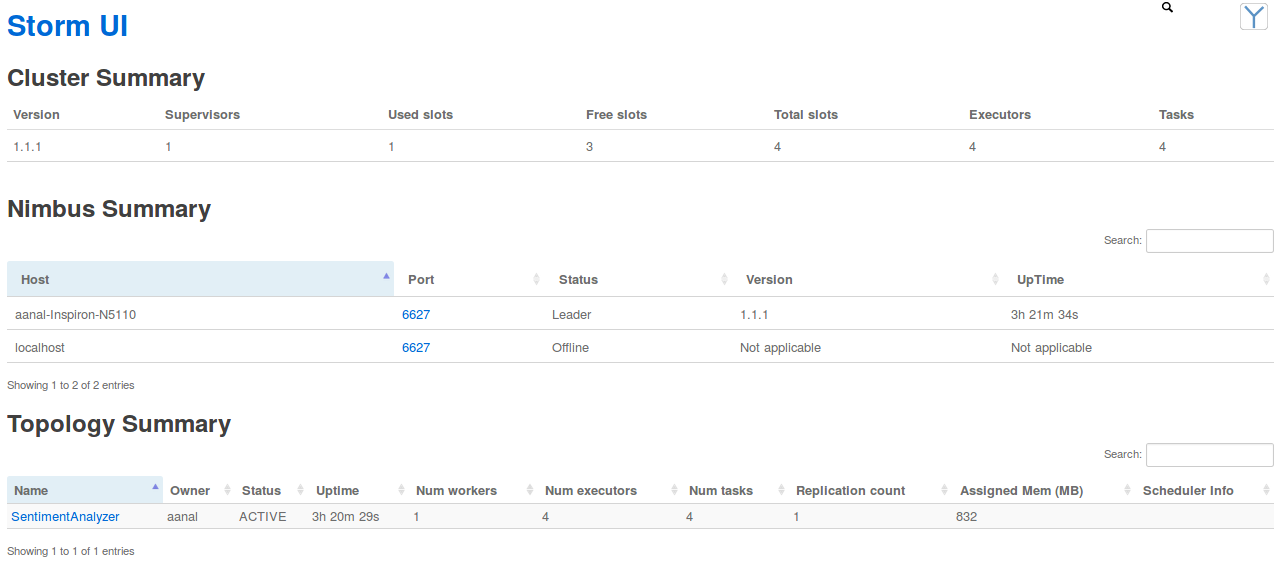
\includegraphics[width=\textwidth]{ui-mainpage.png}
    \caption{Main Page for Storm UI, displays all the cluster related details}
    \label{fig:stormui}
   \end{center}
\end{figure}

\section{Other Tools}
 \label{sec:othertools}
Stream processing is a topic under constant focus at present and a lot of tools as well as models have been designed and created to support it. This section makes a comparison of the available widely accepted tool today. The available tools are mentioned below in brief such as:
 
 \begin{enumerate}
 \item \textbf{Spark Streaming} is an Open Source based project for stream processing.  It relies on cluster computing systems and operates on batches. The batch window in Spark Streaming is comparatively small thus allowing stream processing.It also provides flexibility to work in different programming languages such as Java, Scala and Python.
 \item \textbf{Apache Samza} is an Open Source project for near realtime distributed stream processing framework. It uses Apache Kafka for messaging and Apache Hadoop YARN for fault tolerance, processor isolation, security and resource management.\footnote{http://samza.apache.org/}
 \item \textbf{Flink Streaming} is also a Real time stream processing tool for distributed systems and builds batch processing on top of the Streaming engine.
 \end{enumerate}
 
 \subsection{Comparison between Storm, Spark and Samza}
This sub section compares the three most widely used tools for Stream Processing, i.e. Storm, Spark and Samza. 
 
 \subsubsection{Development and Testing}
All three tools provide their own API for development and testing. A comparision among these tools can be made on a basis of the programming languages supported, Apache Samza currently only supports JVM languages, whereas Spark Streaming supports Java, Scala and Python. Apache Storm on the other hand supports JVM as well as Non JVM languages which increases development speed, as the developers can choose their language according to their comfort. Apart from the fact that choosing a language for development, users can utilize existing code, thus allowing high portability.
 
 \subsubsection{Tool setup}
Setting up of the tool in Apache Storm required minimum effort, achieved by downloading the zookeeper and storm binaries and unpacking them onto the computer. A minor configuration changes required attention, such as the location where zookeeper and storm would store data in. Apart from these details, it worked perfectly out of the box. Along the same line, Spark Streaming follows a similar approach for tool setup and can be installed by simply downloading the tarball and unpacking it. Apache Samza on the other hand maintains a repository \url(https://github.com/apache/samza-hello-samza) which contains the scripts which installs and starts the requirement dependencies in the host.
 
 \subsubsection{Deployment}
Deployment of an artifact on Apache storm is relatively easy. For the java application, one compiles the sources with all the required dependencies into a jar file. The jar file can then be easily deployed into storm via a simple command.
 
 \subsubsection{Fault Tolerance}
As stream processing systems run for extended periods, it is quite necessary that these should be able to handle various kinds of faults and still keep processing data as they enter the system. The fault tolerance model for Storm has been extensively described in section \ref{sec:resilience}. Similarly, Spark Streaming and Apache Samza also use various techniques to resolve issues while deployed. Spark Streaming uses write ahead logs(journals) to keep track of all the data operation, and during failure of a worker, the worker is restarted and a state restore is done by reading the logs. This ensures that the data is processed as required. In comparison to Apache Storm, Storm continues to process incoming tuples even when the master node fails, but in Spark, the worker nodes stop working when the master node fails until a new leader starts. This is an added bonus to Storm, since a failed master manual restart would reinstate the state of the system without many changes.

\begin{figure}
\begin{center}
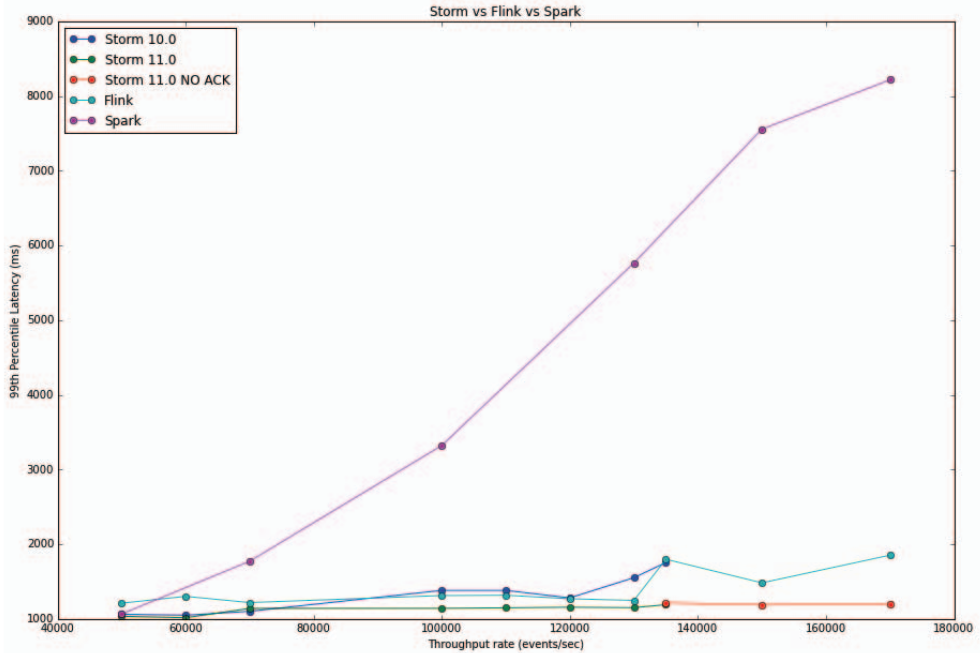
\includegraphics[width=.75 \textwidth]{comparisiongraph.png}
\caption{Performance Comparision between Apache Storm, Apache Flink and Spark Streaming \cite{benchmark}}
\label{fig:comparisiongraph}
\end{center}
\end{figure}
 
 \subsubsection{Benchmarks}
There have not been a comparative benchmark between Apache Storm, Spark Streaming and Apache Samza, but various sources have different comparisions between tools.  \cite{benchmark} considers Apache Storm, Spark Streaming and Apache Flink. The benchmark design consisted of counting the number of events taking place in the stream. The design was setup to read data from a Kafka Event Queue, the data being processed and result updated into Redis. The result included the window start time and the window end time, thus giving  an idea about the total latency of processing. According to this benchmark, they deduced that Apache Storm and Flink had low latency, whereas Spark Streaming had higher maximum throughput depending upon the batch duration setting. Figure \ref{fig:comparisiongraph} shows the comparative analysis among Apache Flink, Spark Streaming and Apache Storm. The batch processing scheme of Spark Streaming allows it to process events with higher throughput but with a trade off that the processing is delayed with higher latency. In the figure, we can observe that storm has comparatively less delay in processing, but according to \cite{benchmark}, storm with acking beyond 135,000 events per second, could not keep up with the throughput.
 
 \section{Discussion}
Apache Storm acts as a real time stream processing tool which is capable of computing results with high reliability and minimum latency. The tool is comparatively easy to setup and configure, with out of the box configurations which is production ready. The storm API is relatively simple and does not have a complicated method calls, the programming is based on event driven programming and since storm supports read and writes based on standard IO, utilizing previously written code could be relatively easier than in the other available tools. Data is currently being generated and consumed at an unprecedented rate, thus stream processing technologies is a requirement and is gaining popularity and attention. With all the various tools available, one can decide on which tool best suites ones needs. According to the benchmarks, if minimum latency is required, Apache Storm or Apache Flink or any system with Continuous data flow model should be preferred. Whereas if high throughput is required with a non strict latency criteria, Spark streaming could prove to be a better option.


%%%%%%%%%%%%%%%%%%%%%%%%%%%%%%%%%%%%%%%%%%%%%%%%%%%%%%%%%%%%%%%%%%%%%%%%%%%%%%%

\section{Bibliography}
\bibliographystyle{splncs03}
\bibliography{paper}
All Links were verified at 10.01.2018
\end{document}
